\let\negmedspace\undefined
\let\negthickspace\undefined
\documentclass[journal]{IEEEtran}
\usepackage[a5paper, margin=10mm, onecolumn]{geometry}
%\usepackage{lmodern} % Ensure lmodern is loaded for pdflatex
\usepackage{tfrupee} % Include tfrupee package

\setlength{\headheight}{1cm} % Set the height of the header box
\setlength{\headsep}{0mm}     % Set the distance between the header box and the top of the text

\usepackage{gvv-book}
\usepackage{gvv}
\usepackage{cite}
\usepackage{amsmath,amssymb,amsfonts,amsthm}
\usepackage{algorithmic}
\usepackage{graphicx}
\usepackage{textcomp}
\usepackage{xcolor}
\usepackage{txfonts}
\usepackage{listings}
\usepackage{enumitem}
\usepackage{mathtools}
\usepackage{gensymb}
\usepackage{comment}
\usepackage[breaklinks=true]{hyperref}
\usepackage{tkz-euclide} 
\usepackage{listings}
% \usepackage{gvv}                                        
\def\inputGnumericTable{}                                 
\usepackage[latin1]{inputenc}                                
\usepackage{color}                                            
\usepackage{array}                                            
\usepackage{longtable}                                       
\usepackage{calc}                                             
\usepackage{multirow}                                         
\usepackage{hhline}                                           
\usepackage{ifthen}                                           
\usepackage{lscape}
\begin{document}

\bibliographystyle{IEEEtran}
\vspace{3cm}

\title{9-9.2-25}
\author{EE24BTECH11051 - Prajwal}
% \maketitle
% \newpage
% \bigskip
{\let\newpage\relax\maketitle}

\renewcommand{\thefigure}{\theenumi}
\renewcommand{\thetable}{\theenumi}
\setlength{\intextsep}{10pt} % Space between text and floats


\numberwithin{equation}{enumi}
\numberwithin{figure}{enumi}
\renewcommand{\thetable}{\theenumi}
\textbf{Question}:\\
Using integration, find the area of the region bounded by the parabolas $y^2\;=\;4x$ and  $x^2\;=\;4y$.
\\
\solution
\begin{table}[h!]    
  \centering
  \begin{center}
    \begin{tabular}{|c|c|c|} 
        \hline
            \textbf{Variable} & \textbf{Description} & \textbf{Formula} \\ 
        \hline
            $A$   & It is one end of the line segment & $\myvec{5 \\ -6}$ \\ 
        \hline
            $B$   & It is other end of line segment &  $\myvec{-1\\-4}$\\ 
        \hline
            $C$   & It is the point of intersection of line segment and $Y$-axis & $C  = \myvec{0\\y}$\\ 
        \hline
        
    \end{tabular}
\end{center}  

  \caption{Variables Used}
  \label{tab1-1.2-20}
\end{table}
The parameters of the conics are
\begin{align}
V_1=\myvec{0 & 0 \\ 0 & 1}\;,\;u_1=\myvec{-2\\0} \;,\;f_1=0\\
V_2=\myvec{1 & 0 \\ 0 & 0}\;,\;u_2=\myvec{0\\-2}\;,\;f_2=0
\end{align}
The intersection of two conics with parameters $V_i,u_i,f_i,\;i= 1,2$ is defined as
\begin{align}
x^T\brak{V_1+\mu V_2}x+2\brak{u_1+\mu u_2}^T x + \brak{f_1+\mu f_2}\;=\;0
\end{align}
Solving this the points of intersection are
\begin{align}
\myvec{0\\0}\;,\;\myvec{4\\4}
\end{align}
Area between the curves is,
\begin{align}
\int_{0}^{4} \brak{\sqrt{4x}-\frac{x^2}{4}} \, dx 
\end{align}
By solving the integration, we get area is equal to 5.33 sq.units
\begin{figure}[h!]
   \centering
   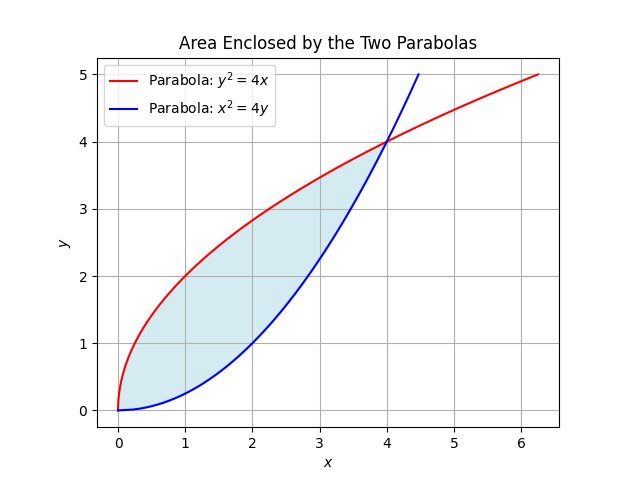
\includegraphics[width=\linewidth]{figs/Figure_1.png}
   \label{stemplot}
   \caption{}
\end{figure}





\end{document}
